\documentclass[conference]{IEEEtran}
\IEEEoverridecommandlockouts

\usepackage[utf8]{inputenc}
\usepackage{mathptmx}
\usepackage{enumitem}
\usepackage{hyperref}
\usepackage{url}
\usepackage{graphicx}
\usepackage{caption}
\usepackage{subcaption}
\usepackage{float}
\usepackage{amsmath}
\usepackage{amsfonts}
\usepackage{amssymb}
\usepackage{multirow}
\usepackage{tabularx}
\usepackage{comment}
\usepackage{balance}

\def\BibTeX{{\rm B\kern-.05em{\sc i\kern-.025em b}\kern-.08em
    T\kern-.1667em\lower.7ex\hbox{E}\kern-.125emX}}

\setlength{\textfloatsep}{6pt plus 2pt minus 2pt}
\setlength{\floatsep}{6pt plus 2pt minus 2pt}
\setlength{\intextsep}{5pt plus 2pt minus 2pt}
\setlength{\abovecaptionskip}{3pt}
\setlength{\belowcaptionskip}{2pt}

\begin{document}

\title{AdaPart-GNN: Scale-Adaptive Graph Partitioning with Boundary Prompting for Scalable GNNs}

\author{
\IEEEauthorblockN{Surendra Kumar Raut}
\IEEEauthorblockA{\textit{Department of CSE} \\
IIT Bhilai, India \\
surendrakr@iitbhilai.ac.in}
\and 	
\IEEEauthorblockN{Kishan Tamboli}
\IEEEauthorblockA{\textit{Department of CSE} \\
IIT Bhilai, India \\
kishant@iitbhilai.ac.in}
\and
\IEEEauthorblockN{Vishwesh Jatala}
\IEEEauthorblockA{\textit{Department of CSE} \\
IIT Bhilai, India \\
vishwesh@iitbhilai.ac.in}
}

\maketitle

\begin{abstract}
Nowadays, large-scale graph processing is performed using Graph Neural Networks (GNNs) to find patterns in graph-structured data; however, it faces severe memory and computational bottlenecks during training. As a remedy, partition-based training reduces GPU memory by dividing graphs into smaller subgraphs and training them sequentially, but discarding inter-partition edges causes information loss and accuracy degradation. Moreover, fixed partition configurations may lead to inefficient GPU memory utilization.

To overcome these challenges, we introduce AdaPart-GNN, an efficient and boundary-preserving framework for large-scale GNN training. AdaPart-GNN first determines a scale-adaptive partition count ($K^*$) based on graph characteristics and GPU memory constraints. Second, it employs Jaccard-Eigenvector weighting to identify and preserve structurally dense communities during graph partitioning. Finally, a lightweight Boundary Eigen-Prompt module injects topological prompts into boundary nodes, restoring severed cross-partition signals without communication. Experiments on five benchmark datasets show up to 31.2$\times$ speedup (16.5$\times$ average) over DGL GraphSAGE, up to 64.4\% peak VRAM reduction, +11.7\% accuracy on Ogbn-arxiv, and +13.2\% Micro-F1 on Yelp.
\end{abstract}


\section{Introduction}
Graph Neural Networks (GNNs) are the foundational paradigm for machine learning on relational structures. However, recursive multi-hop message passing triggers the well-known \textit{neighborhood explosion} problem: receptive fields expand exponentially with network depth, resulting in prohibitive computation and memory footprints that exceed commodity GPU memory.

To scale GNN training, two primary strategies exist: stochastic neighbor sampling (e.g., GraphSAGE~\cite{graphsage}), which bounds neighborhood sizes but incurs redundant data movement and high sampling latency; and Subgraph sampling (e.g., Cluster-GCN~\cite{cluster_gnn}), which divides the graph into subgraphs and trains mini-batches strictly within partitions.

While partitioning bounds peak VRAM to partition size and avoids redundant transfers, it suffers from the \textit{boundary cut-edge dilemma}: severing cross-partition edges isolates boundary nodes from essential neighborhood messages, degrading representation quality on relational graphs. Furthermore, rigid, topology-oblivious partition counts ($K$) cause either GPU Out-Of-Memory (OOM) exceptions or excessive edge cuts.

To overcome these challenges, we propose \textbf{AdaPart-GNN}, an efficient, scale-adaptive, and boundary-preserving GNN training framework. Our contributions are three-fold:
\begin{itemize}[leftmargin=*,noitemsep,topsep=1pt]
    \item \textbf{Scale-Adaptive Partitioning}: An analytical heuristic ($K^*$) that determines the partition count based on graph scale, structural density, and GPU memory limits.
    \item \textbf{Jaccard-Eigenvector Edge Weighting}: A hybrid metric combining local cohesion and eigenvector centrality to guide METIS toward preserving vital dense communities.
    \item \textbf{Boundary EigenPrompt Bridging}: A parameter-efficient prompt module restoring cross-partition topological awareness for cut nodes without inter-subgraph communication.
\end{itemize}

Across five diverse benchmarks, AdaPart-GNN achieves an average speedup of \textbf{16.5$\times$} over DGL (GraphSAGE), slashes peak GPU memory by up to \textbf{64.4\%}, and boosts test accuracy by up to \textbf{+11.7\%} over unweighted partition baselines.


\section{Approach} \label{sec:approach}
AdaPart-GNN addresses scalability and accuracy trade-offs in partition-based GNNs via three synergistic stages: (1) scale-adaptive partition determination, (2) Jaccard-eigenvector edge weighting, and (3) boundary prompt bridging (Figure~\ref{fig:approach}).

\textbf{1) Scale-Adaptive Partition Sizing ($K^*$):}
Fixed partition counts cause Out-Of-Memory (OOM) failures on massive graphs or severe community disruption on smaller graphs. To balance hardware limits with topological fidelity, we formulate a scale- and density-aware sizing heuristic:
{\setlength{\abovedisplayskip}{2pt}\setlength{\belowdisplayskip}{2pt}
\begin{equation} \label{eq:kstar}
K^* = \left\lceil \frac{|V|}{N_{\text{target}}} \cdot \left(1 + \beta \log_{10}\left(1 + \frac{2|E|}{|V|}\right)\right) \right\rceil
\end{equation}}
where $N_{\text{target}} \approx \frac{M_{\text{gpu}}}{\text{Mem}_{\text{node}}} \approx 35{,}000\text{--}40{,}000$ is the hardware-budgeted node capacity per subgraph ($\le 1.5$\,GB GPU allocation, accommodating feature tensors and SpMM buffers), setting $\frac{|V|}{N_{\text{target}}}$ as the baseline partition count. The average degree $\frac{2|E|}{|V|}$ measures structural density, penalizing edge-heavy graphs where message passing inflates activation memory, while $\log_{10}$ dampens power-law skews ($\beta \approx 0.35$). Intuitively, Equation~\eqref{eq:kstar} scales $K^*$ on massive graphs ($K^*=69$ on Products) to avoid OOMs while preserving relational structure on smaller graphs ($K^*=13$ on Arxiv).

\begin{figure}[t]
    \centering
    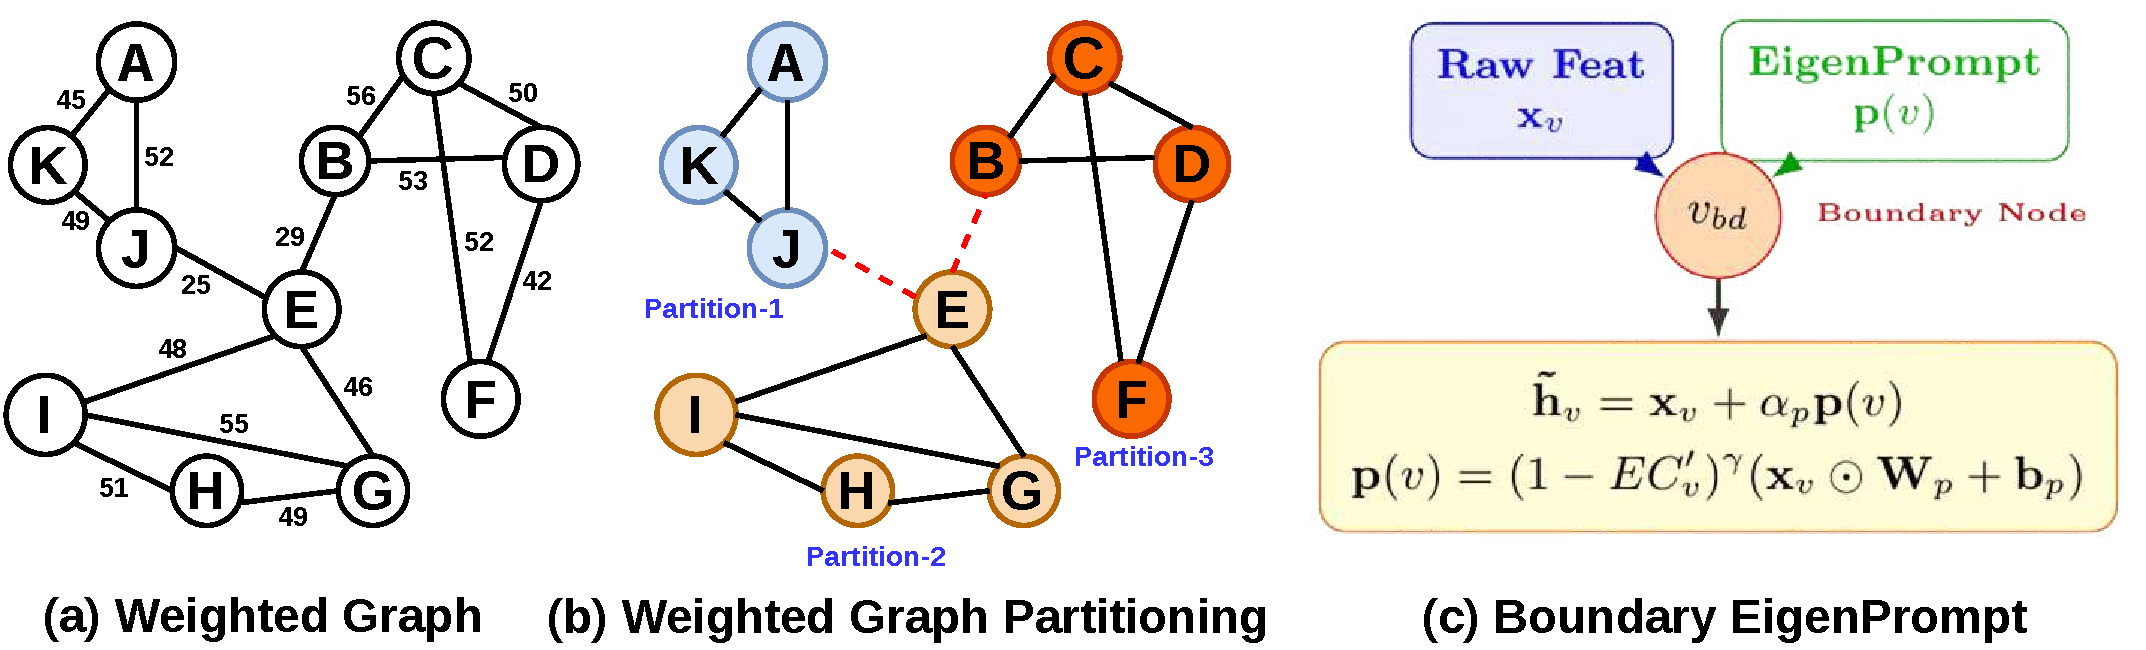
\includegraphics[width=0.98\columnwidth]{image/problem3_overview.pdf}
    \vskip 1mm
    \caption{AdaPart-GNN framework: (a) Weighted Graph, (b) Weighted Graph Partitioning with severed cuts, and (c) Boundary EigenPrompt bridging.}
    \label{fig:approach}
\end{figure}

\textbf{2) Jaccard-Eigenvector Edge Weighting:}
Standard METIS partitioning minimizes unweighted cuts, severing vital dense communities. To retain high-centrality pathways, we formulate a composite similarity combining neighborhood overlap (Jaccard) with global influence (eigenvector centrality):
{\setlength{\abovedisplayskip}{2pt}\setlength{\belowdisplayskip}{2pt}
\begin{equation} \label{eq:weight}
S_{uv} = J_{uv}^\alpha \cdot \left(\sqrt{EC'_u \cdot EC'_v}\right)^{1-\alpha}, \quad w_{uv} = 1 + \left\lfloor K_{\text{scale}} \cdot S_{uv} \right\rceil
\end{equation}}
where $J_{uv} = \frac{|N(u) \cap N(v)|}{|N(u) \cup N(v)|}$ captures community cohesion, and $EC'_v = \frac{EC_v}{\max_{k} EC_k} \in [0, 1]$ is the normalized eigenvector centrality. We empirically set $\alpha = 0.7$, balancing local cohesion with global topology while keeping $S_{uv} \in [0, 1]$. To satisfy METIS integer requirements, $w_{uv} = 1 + \text{round}(K_{\text{scale}} S_{uv})$ ($K_{\text{scale}} = 100$) maps weights to $[1, 101]$, guiding METIS to preserve cohesive partitions and cutting boundary loss by up to 8.1\% on Reddit.

% =========================================================================
% PREVIOUS VERSIONS (COMMENTED OUT FOR EASY RESTORATION IF NEEDED)
% =========================================================================
% \textbf{3) Boundary EigenPrompt Bridging:}
% Partitioning severs cross-partition edges during subgraph-batch training, starving boundary nodes $v \in \mathcal{V}_{bd}$ of global context. Cross-partition feature transfer incurs heavy communication latency. To compensate for lost global information with zero communication, we inject a Boundary EigenPrompt $\mathbf{p}(v)$ into node features $\mathbf{x}_v$:
% {\setlength{\abovedisplayskip}{2pt}\setlength{\belowdisplayskip}{2pt}
% \begin{equation} \label{eq:prompt}
% \mathbf{\tilde{h}}_v = \mathbf{x}_v + \alpha_p \cdot \mathbf{p}(v), \quad \mathbf{p}(v) = (1 - EC'_v)^\gamma \cdot (\mathbf{x}_v \odot \mathbf{W}_p + \mathbf{b}_p)
% \end{equation}}
% where learnable weights and biases $\mathbf{W}_p, \mathbf{b}_p \in \mathbb{R}^D$ are shared globally across all subgraphs to learn a global topological prior without inter-subgraph communication. The factor $(1 - EC'_v)^\gamma$ forms a topological boundary gate with empirically chosen $\gamma = 1.5$, providing super-linear suppression of prompt noise on semi-central nodes while fully activating on peripheral cut nodes ($EC'_v \approx 0$). For interior hubs ($EC'_v \approx 1$), the gate vanishes ($(1 - EC'_v)^\gamma \to 0$). With $\alpha_p$ scaling prompt strength and only $\mathcal{O}(D)$ parameters ($<6$\,MB overhead), this restores relational context with zero runtime communication.
% =========================================================================

\textbf{3) Boundary EigenPrompt Bridging:}
When a graph is partitioned, boundary nodes lose connections to neighbors in other partitions. While transferring cross-partition features restores this context, it causes heavy communication overhead. To solve this with zero communication, we inject a lightweight \textit{Boundary EigenPrompt} $\mathbf{p}(v)$ directly into node features $\mathbf{x}_v$:
{\setlength{\abovedisplayskip}{2pt}\setlength{\belowdisplayskip}{2pt}
\begin{equation} \label{eq:prompt}
\mathbf{\tilde{h}}_v = \mathbf{x}_v + \alpha_p \cdot \mathbf{p}(v), \quad \mathbf{p}(v) = (1 - EC'_v)^\gamma \cdot (\mathbf{x}_v \odot \mathbf{W}_p + \mathbf{b}_p)
\end{equation}}
Here, $\mathbf{W}_p, \mathbf{b}_p \in \mathbb{R}^D$ are learnable vectors shared across subgraphs to provide global context, and $\alpha_p$ is a scaling factor ensuring the prompt supplements rather than overpowers original node features $\mathbf{x}_v$. The term $(1 - EC'_v)^\gamma$ adaptively modulates prompt strength based on node centrality: isolated boundary nodes ($EC'_v \approx 0$) receive full prompt compensation, while well-connected interior hubs ($EC'_v \approx 1$) receive near-zero prompt ($(1 - EC'_v)^\gamma \to 0$) to protect intact features. Setting $\gamma = 1.5$ smoothly suppresses prompt noise on moderately connected nodes. Since only $\mathbf{W}_p$ and $\mathbf{b}_p$ are trained, the entire prompt module and its optimizer states consume $<6$\,MB of GPU memory, restoring boundary accuracy with zero runtime communication.

\section{Experimental Evaluation}

We performed our experiments on a single NVIDIA RTX A6000 GPU (48\,GB), Intel Xeon Gold 5218 CPU (16 cores), and 512\,GB RAM with PyTorch 2.1 and DGL 2.4.0. Evaluated datasets, properties, and adaptive partitions ($K^*$) are summarized in Table~\ref{tbl:results}. Results use a 3-layer GraphSAGE (dim 256, LayerNorm, Adam lr 0.001, 100 epochs).

\textbf{Comparison with State-of-the-Art:}
As reported in Table~\ref{tbl:results}, AdaPart-GNN outperforms state-of-the-art stochastic sampling (DGL GraphSAGE~\cite{graphsage}) and Subgraph sampling (METIS~\cite{metis}), reaching up to \textbf{31.2$\times$} speedup on Yelp and \textbf{25.0$\times$} on IGB-small (\textbf{16.5$\times$} average) over DGL GraphSAGE due to: (1) eliminating redundant neighbor sampling and transfers, and (2) scale-adaptive sizing ($K^*$), optimizing GPU residency and SpMM throughput vs. Subgraph sampling (METIS).

\begin{table}[t]
\centering
\caption{Comparison with DGL (GraphSAGE) and Subgraph sampling (METIS) ($M$: million; Micro-F1 in brackets for Yelp).}
\label{tbl:results}
\renewcommand{\arraystretch}{0.92}
\resizebox{\columnwidth}{!}{%
\begin{tabular}{|l|c|c|c|l|r|r|r|}
\hline
\multicolumn{1}{|c|}{\textit{\textbf{Dataset}}} &
  \textit{\textbf{$|V|$}} &
  \textit{\textbf{$|E|$}} &
  \textit{\textbf{$K^*$}} &
  \multicolumn{1}{c|}{\textit{\textbf{Metrics}}} &
  \multicolumn{1}{c|}{\textit{\textbf{DGL (SAGE)}}} &
  \multicolumn{1}{c|}{\begin{tabular}[c]{@{}c@{}}\textit{\textbf{Subgraph sampling}}\\\textit{\textbf{(METIS)}}\end{tabular}} &
  \multicolumn{1}{c|}{\textit{\textbf{AdaPart-GNN}}} \\ \hline

\multirow{2}{*}{\begin{tabular}[c]{@{}l@{}}Ogbn-\\arxiv\end{tabular}} 
  & \multirow{2}{*}{0.17M} & \multirow{2}{*}{1.17M} & \multirow{2}{*}{13}
  & Train Time (s) & 127.11 & 17.48 (7.3$\times$) & \textbf{11.42 (11.1$\times$)} \\ \cline{5-8}
  & & & & Accuracy & 0.56 & 0.55 & \textbf{0.67 (+11\%)} \\ \hline

\multirow{2}{*}{Reddit} 
  & \multirow{2}{*}{0.23M} & \multirow{2}{*}{114.6M} & \multirow{2}{*}{17}
  & Train Time (s) & 633.18 & \textbf{60.27 (10.5$\times$)} & 61.19 (10.4$\times$) \\ \cline{5-8}
  & & & & Accuracy & \textbf{0.96} & 0.94 & 0.94 \\ \hline

\multirow{2}{*}{Yelp} 
  & \multirow{2}{*}{0.72M} & \multirow{2}{*}{13.95M} & \multirow{2}{*}{26}
  & Train Time (s) & 1687.25 & 59.10 (28.6$\times$) & \textbf{54.15 (31.2$\times$)} \\ \cline{5-8}
  & & & & Acc (Micro-F1) & 0.92 (0.41) & 0.92 (0.35) & \textbf{0.93 (0.48)} \\ \hline

\multirow{2}{*}{\begin{tabular}[c]{@{}l@{}}IGB-\\small\end{tabular}} 
  & \multirow{2}{*}{1.00M} & \multirow{2}{*}{12.07M} & \multirow{2}{*}{32}
  & Train Time (s) & 4259.40 & \textbf{170.01 (25.1$\times$)} & 170.58 (25.0$\times$) \\ \cline{5-8}
  & & & & Accuracy & 0.74 & 0.75 & \textbf{0.76} \\ \hline

\multirow{2}{*}{\begin{tabular}[c]{@{}l@{}}Ogbn-\\products\end{tabular}} 
  & \multirow{2}{*}{2.45M} & \multirow{2}{*}{61.86M} & \multirow{2}{*}{69}
  & Train Time (s) & 717.15 & 149.05 (4.8$\times$) & \textbf{140.39 (5.1$\times$)} \\ \cline{5-8}
  & & & & Accuracy & 0.78 & 0.77 & \textbf{0.79} \\ \hline
\end{tabular}%
}
\end{table}


\begin{figure}[t]
\centering
\begin{minipage}{.24\textwidth}
  \subfloat[EigenPrompt Ablation]{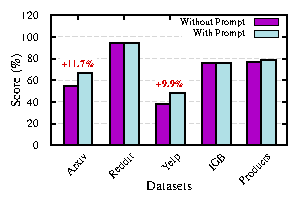
\includegraphics[width=\linewidth]{image/fig_accuracy.pdf}\label{fig:accuracy}}
\end{minipage}%
\hfill
\begin{minipage}{.24\textwidth}
  \subfloat[Peak VRAM Footprint]{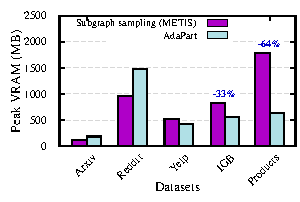
\includegraphics[width=\linewidth]{image/fig_vram.pdf}\label{fig:vram}}
\end{minipage}
\caption{(a) EigenPrompt ablation (Accuracy; Micro-F1 for Yelp), and (b) Peak VRAM vs. Subgraph sampling (METIS) ($K=20$).}
\label{fig:ablation}
\end{figure}

\pagebreak
\textbf{Peak Memory Scalability:}
As shown in Figure~\ref{fig:ablation}(b), adaptive sizing ($K^*$) cuts peak VRAM by \textbf{64.4\%} on Ogbn-products (1,788.7\,MB to \textbf{635.9\,MB}) and \textbf{33.3\%} on IGB-small vs. Subgraph sampling (METIS) ($K=20$). For smaller graphs, $K^*$ avoids over-fragmentation, fitting budget GPUs ($\le 1.5$\,GB) while preserving topology.

\textbf{Effect of Boundary EigenPrompt (Ablation):}
To isolate Boundary EigenPrompt's impact, Figure~\ref{fig:ablation}(a) compares AdaPart-GNN (With Prompt) against unprompted training (Without Prompt, $\mathbf{p}(v)=\mathbf{0}$). Prompting recovers severed context on cut-sensitive graphs, boosting accuracy by \textbf{+11.7\%} on Ogbn-arxiv (to \textbf{66.78\%}) and Micro-F1 by \textbf{+9.9\%} on Yelp (to \textbf{48.15\%}). On dense graphs (Reddit), the boundary gate $(1-EC'_v)^\gamma$ attenuates prompting with $<6$\,MB memory overhead and zero latency.


%\balance
\section{Conclusion} \label{sec:conclusion}
We proposed AdaPart-GNN, an efficient partitioning framework for scalable GNN training. By combining adaptive partition sizing ($K^*$), edge weighting, and Boundary EigenPrompt bridging, AdaPart-GNN eliminates cross-partition communication while recovering structural context. It achieves up to \textbf{31.2$\times$} speedup over DGL (GraphSAGE) and \textbf{64.4\%} peak VRAM reduction, with consistent accuracy gains (+11.7\% on Arxiv). Future work explores distributed multi-GPU scaling.



\bibliographystyle{IEEEtran}
\bibliography{References/ref}

\end{document}
